% !TeX root = ../praktikum.tex
% !TeX encoding = UTF-8
% !Tex spellcheck = de_DE


Im letzten Versuchsteil wird der Laserstrahl am anderen Ende der lichtleitenden Faser ausgekoppelt und auf einen optischen Pfad gesandt, um ihn zur Messung von Abbildungen von Objekten und deren Fourierspektren zu verwenden.
Hinter dem Faserauskoppler wird der Aufbau aus Abbildung \ref{fig:4f-aufbau} realisiert. \\

\begin{figure}[h]
\centering
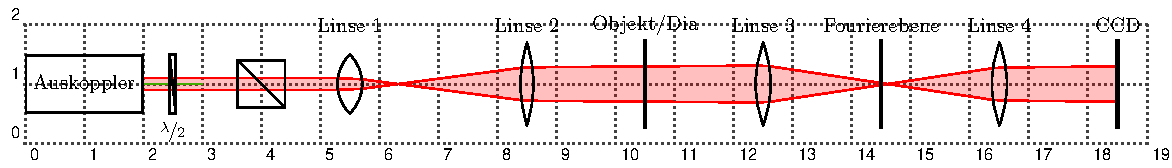
\includegraphics[width=0.7\linewidth]{graphs/versuchsaufbau/4f-aufbau}
\caption{Schematische Skizze des 4f-Aufbaus. Der Laserstrahl passiert nach verlassen des Auskopplers eine $\frac{\lambda}{2}$- Platte und anschließend einen Strahlteiler. Der zweite Teil des Strahls, welcher vom Strahlteiler abgelenkt wird, trifft auf eine Strahlblockierung und wird nicht weiter verwendet. Zwischen Linse 2 und 3 befindet sich die Halterung für das Objekt/Dia, in der Fourierebene wird entweder eine zweite Kamera oder ein Filter positioniert. Die CCD Kamera am Ende des Strahlengangs befindet sich in der Abbildungsebene des Aufbaus.}
\label{fig:4f-aufbau}
\end{figure}

In dem hier verwendeten, sogenannten 4f-Aufbau passiert der Laserstrahl nach der Reflektion am ersten Spiegel eine $\frac{\lambda}{2}$- Platte und dahinter einen Strahlteiler. Mithilfe dieser beiden Komponenten kann die Intensität des anschließend verwendeten Strahls eingestellt werden. \\
Um die abzubildenden Objekte vollständig ausleuchten zu können, wird der Laserstrahl mithilfe der ersten beiden Linsen aufgeweitet und wieder kollimiert. Im Brennpunkt der dritten Linse befindet sich ein Objektträger in der Gegenstandsebene. In diesem werden die abzubildenden Objekte angebracht. \\
Die Fourierebene befindet sich im Brennpunkt der Linsen 3 und 4. Nach der vierten Linse wird der Strahl erneut kollimiert und trifft auf die CCD Kamera, Kamera 1. \\
Um Aufnahmen der Fourierspektren zu erhalten, wird bei Bedarf eine zweite Kamera, Kamera 2, in der Fourierebene montiert. \\ 

Verwendet wurden hierbei Linsen der Brennweiten wie folgt: Linse 1 mit $f_{1}=20mm$ , Linse 2 mit $f_{2}=300mm$ , Linse 3 mit $f_{3}=100mm$ , Linse 4 mit $f_{4}=100mm$ .
Direkt hinter dem Auskoppler wurde zusätzlich ein Spiegel, reflektierend für Wellenlängen zwischen 400 - 700 nm, in den 4f-Aufbau aufgenommen, um den Verlauf des Laserstrahls im optischen Pfad besser feinjustieren zu können. Ebenso wurde ein Pinhole im Fokus der Linsen 1 und 2 ergänzt, um das Gaußprofil des zur Messung verwendeten Laserstrahls zu optimieren, da dieses durch den zusätzlich eingesetzten Spiegel an Qualität verlor. \\

Nachdem der 4f-Aufbau montiert und der Verlauf des Laserstrahls im optischen Pfad optimiert ist, werden nacheinander die Objekte 1 bis 5 (Siehe Abbildung \ref{fig:Objekte-aus-Anleitungsheft}) in Form von Dias in dem Objektträger montiert. 
\begin{figure}
\centering
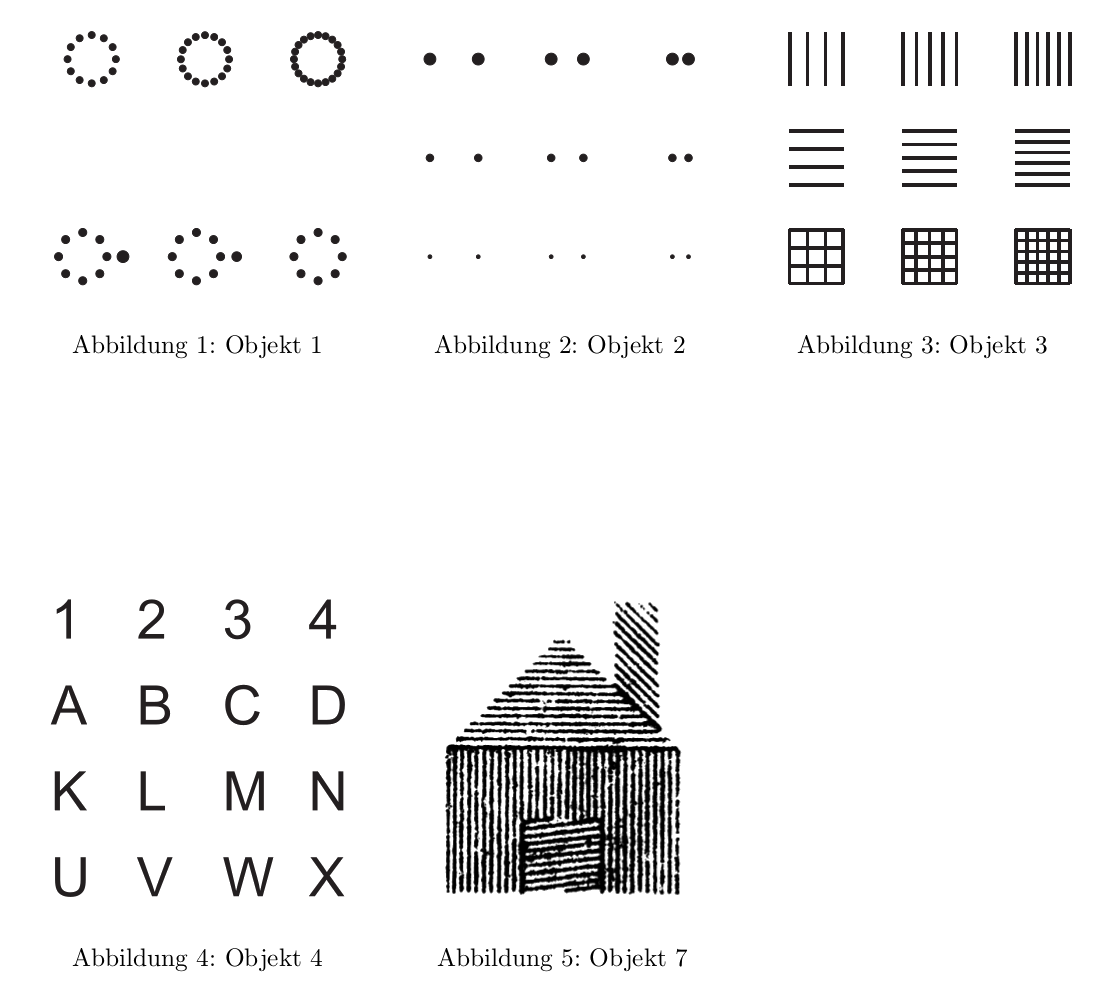
\includegraphics[width=0.7\linewidth]{images/Anleitungsheft/Objekte-aus-Anleitungsheft}
\caption{Darstellung der zur Messung verwendeten Dias}
\label{fig:Objekte-aus-Anleitungsheft}
\end{figure}

Anhand der Dias werden zunächst sowohl Kamera 1, als auch Kamera 2 nachjustiert, bis ein möglichst scharfes Bild auf dem über das Programm \textit{uc480 Viewer-DCC1545M-ID} angeschlossenen Bildschirm zu erkennen ist.  \\
Mit den beiden Kameras werden nacheinander für jedes der Objekte Aufnahmen in der Abbildungsebene und zugehörig zu jeder Einstellung auch in der Fourierebene gemacht. Zudem werden für die Objekte 4 und 5 beispielhaft verschiedene Filter in die Fourierebene gestellt und Aufnahmen der Kamera 1 in der Abbildungsebene gemacht. Für Objekt 4 wird hierzu ein Tiefpass und mehrere Breitbandfilter verwendet. Für Objekt 5 wird ein Halbebenenfilter horizontal, vertikal und diagonal in die Fourierebene gehalten. \\

Als Nächstes wird die Abbildung eines Fingerabdrucks auf einem Glasplättchen zunächst ohne Filter aufgenommen. Anschließend wird die Abbildung mit einem in der Fourierebene befindlichen Hochpass- und einem Halbebenenfilter aufgenommen. Zudem wird mit Kamera 2 das Fourierspektrum des Fingerabdrucks photographiert. \\

Als Letztes wird ein Teelicht auf die Position des Objektträgers gestellt und ein Halbebenenfilter in der Fourierebene installiert. Mit Kamera 1 werden mehrere Abbildungen aufgenommen, um die Strömungsbewegungen oberhalb der Flamme beobachten zu können. 
Zum Vergleich wird zudem eine Aufnahme mit Halbebenenfilter, jedoch ohne Teelicht gemacht. 





